\documentclass[conference]{IEEEtran}
\IEEEoverridecommandlockouts

\usepackage{cite}
\usepackage{amsmath,amssymb,amsfonts}
\usepackage{graphicx}
\usepackage{textcomp}
\usepackage{xcolor}
\usepackage{array}
\usepackage{booktabs}
\usepackage{tabularx}
\usepackage{tikz}
\usetikzlibrary{arrows.meta,positioning,fit,calc,shapes.geometric}
\usepackage{pgfplots}
\pgfplotsset{compat=1.18}
\usepackage[hidelinks]{hyperref}

% Lets the author block wrap onto a second row (five authors: three + two).
\makeatletter
\newcommand{\linebreakand}{%
  \end{@IEEEauthorhalign}
  \hfill\mbox{}\par
  \mbox{}\hfill\begin{@IEEEauthorhalign}
}
\makeatother

\newcolumntype{Y}{>{\raggedright\arraybackslash}X}
\tikzset{
  box/.style={draw, rounded corners=1.5pt, align=center, font=\scriptsize, inner sep=2.5pt, minimum height=5.5mm},
  grp/.style={draw, dashed, rounded corners=2pt, inner sep=3pt},
  arr/.style={-{Stealth[length=1.6mm]}, semithick},
  human/.style={box, fill=black!8, line width=0.7pt},
}

\begin{document}

\title{Explainable and Risk-Aware Cyber Threat Detection: A Review of Machine Learning, Behavioural Detection, and Human-in-the-Loop Response}

\author{
\IEEEauthorblockN{Ashish Shakya}
\IEEEauthorblockA{Department of Computer Science \& Engineering\\
Sharda School of Computing Science \& Engineering\\
Sharda University, Greater Noida, India\\
ashishrahin@gmail.com}
\and
\IEEEauthorblockN{Satyajeet Kumar}
\IEEEauthorblockA{Department of Computer Science \& Engineering\\
Sharda School of Computing Science \& Engineering\\
Sharda University, Greater Noida, India\\
satyajeetzod@gmail.com}
\and
\IEEEauthorblockN{Ritanshu Kumar}
\IEEEauthorblockA{Department of Computer Science \& Engineering\\
Sharda School of Computing Science \& Engineering\\
Sharda University, Greater Noida, India\\
2023216269.ritanshu@ug.sharda.ac.in}
\and
\IEEEauthorblockN{Swati Singal}
\IEEEauthorblockA{Department of Computer Science \& Engineering\\
Sharda School of Computing Science \& Engineering\\
Sharda University, Greater Noida, India\\
swati.singal@sharda.ac.in}
\and
\IEEEauthorblockN{Mayank Kumar Goyal}
\IEEEauthorblockA{Department of Computer Science \& Engineering\\
Sharda School of Computing Science \& Engineering\\
Sharda University, Greater Noida, India\\
mayank.goyal2@sharda.ac.in}}

\maketitle

\begin{abstract}
Machine-learning threat detectors often score well on benchmark data, yet security analysts still receive alerts they find hard to interpret, rank or act on safely. We treat threat detection broadly, covering malicious processes, ransomware-like file activity and suspicious network behaviour on a host, with network intrusion detection as one part of it. We review 39 sources, foundational works together with studies from 2020 to 2025, covering detection methods, evaluation practice, behavioural ransomware detection, explainability, contextual risk and human-approved response, including recent work on large language models (LLMs). We compare detection approaches, published studies and benchmark datasets, and we re-plot published results to show how much reported scores depend on the feature set and how averaged scores can hide poor detection of rare attack classes. Dataset defects and evaluation pitfalls are well documented but remain common. Explanation methods are seldom tested on whether they help analysts decide, and response automation is mostly studied apart from detection. We assess seven preliminary research gaps, note which are already partly addressed, and outline a conceptual framework that connects detection, contextual risk scoring, explanation, human approval and audit logging. The framework is meant as a starting point for evaluation and has not been validated.
\end{abstract}

\begin{IEEEkeywords}
Threat detection, intrusion detection, anomaly detection, explainable AI, risk assessment, Isolation Forest, ransomware detection, human-in-the-loop security
\end{IEEEkeywords}

%=====================================================================
\section{Introduction}
%=====================================================================
Machine learning (ML) has been applied to detecting cyber attacks for more than two decades, and surveys catalogue dozens of algorithm families evaluated on benchmark data~\cite{buczak2016survey}. Operational adoption has been slower. Sommer and Paxson argued that intrusion detection differs from domains where ML succeeds: attacks are rare, errors are expensive, network traffic is highly diverse, and there is a semantic gap between a statistical outlier and an actionable security event~\cite{sommer2010outside}. More than a decade later, analysts in security operations centres (SOCs) still describe being overwhelmed by alarms that are mostly benign and poorly explained~\cite{alahmadi2022false}, and a study of 30 top-tier security papers found that common ML pitfalls remain widespread~\cite{arp2022dos}. Overviews written from industrial and policy perspectives make related points, stressing the practical problems that affect deployed ML~\cite{apruzzese2022role} and the need to pair AI-driven intrusion detection with organisational and policy measures~\cite{schmitt2025cyber}.

We use \emph{threat detection} in a broader sense than \emph{intrusion detection}. An intrusion detection system (IDS) traditionally looks for unauthorised access or attacks in network traffic or logs~\cite{buczak2016survey}. Threat detection also covers what happens on the host: malicious or unusual processes, ransomware encrypting files, and outbound connections to suspicious destinations~\cite{oz2022survey}. Network intrusion detection is therefore one part of threat detection, and it is the part with the most published benchmarks, which is why much of the evaluation evidence discussed below comes from it.

Detection accuracy, then, is only part of the problem. An analyst also needs to see why an alert was raised, judge how much it matters for the machine involved, and respond without causing new harm. This review is motivated by a final-year project, SecureX, that integrates rule-based, behavioural and anomaly-based detection with contextual risk scoring, plain-language advisories, human-approved containment and audit logging on Windows hosts. The project raised questions that the literature answers only partly, and it is used here only as context; this paper reviews existing research and makes no claim about the project's performance.

We address ten research questions (RQs): how signature-, rule- and anomaly-based methods differ (RQ1); the strengths and limits of Isolation Forest (RQ2); how explainable AI (XAI) helps alert interpretation (RQ3); how contextual risk affects prioritisation (RQ4); the trade-off between automatic and human-approved response (RQ5); how ransomware-like activity can be told apart from legitimate bulk file operations (RQ6); how dataset defects and protocols affect reported results (RQ7); how to evaluate across datasets fairly (RQ8); whether LLMs and retrieval-augmented generation (RAG) can improve explanations while controlling risk (RQ9); and which problems remain open (RQ10).

The contributions are: (i) a comparative synthesis of detection paradigms, published studies and benchmark datasets (Tables~\ref{tab:approaches}--\ref{tab:datasets}); (ii) a re-analysis of published results that illustrates how representation and class imbalance shape reported scores (Figs.~\ref{fig:featuresets}, \ref{fig:imbalance} and~\ref{fig:results}); (iii) an evidence-based assessment of seven preliminary research gaps (Table~\ref{tab:gaps}); and (iv) a conceptual framework and response workflow for explainable, accountable detection (Figs.~\ref{fig:framework} and~\ref{fig:hitl}). Section~II describes the method, Section~III the technical foundations, Section~IV the literature, Section~V the gaps, Section~VI the framework, and Section~VII concludes.

%=====================================================================
\section{Review Methodology}
%=====================================================================
This is a structured narrative review rather than a systematic review. Sources came from two routes. The first was a seed set of 24 papers collected during the SecureX project. Each was read in full and checked against its publisher record; 15 were retained and nine were excluded, seven because their venue, peer-review status or bibliographic metadata could not be verified, one because it was a bachelor's thesis, and one because it addressed smart-city attack advisory, which is outside our scope. The second route was a set of targeted searches carried out in October 2026 through a general web search engine that indexes IEEE Xplore, ACM Digital Library, SpringerLink, ScienceDirect, MDPI, USENIX and arXiv. Queries combined a topic term with a qualifier, for example \textit{(``intrusion detection'' OR ``NIDS'') AND (``dataset'' OR ``evaluation'' OR ``cross-domain'')}, \textit{``ransomware'' AND (``behaviour'' OR ``filesystem'' OR ``detection'')}, \textit{``explainable'' AND (``intrusion detection'' OR ``security'')}, \textit{``alert'' AND (``prioritization'' OR ``fatigue'' OR ``triage'')} and \textit{(``LLM'' OR ``retrieval-augmented'') AND (``cyber security'' OR ``threat intelligence'')}. This route added 24 sources.

We included peer-reviewed papers and clearly labelled preprints that report a method, dataset, evaluation or systematic analysis relevant to an RQ. Studies published between 2020 and 2025 were prioritised, and older work was retained when it introduced a method or dataset still in use. We excluded marketing material, papers whose bibliographic details could not be confirmed, and studies outside host or network detection and response. For every source we recorded authors, venue, year, identifier, objective, method, dataset, metrics and reported results, and every numerical value used in a table or figure was taken directly from the cited table or text. Hit counts per query were not recorded, so we do not report PRISMA-style screening numbers. Fig.~\ref{fig:years} shows the publication years of the 39 included sources. Quality was judged informally from venue, clarity of the evaluation protocol and whether datasets and metrics were reported. Findings were then synthesised by theme, with attention to points where studies agree, disagree or cannot be compared.

\begin{figure}[t]
\centering
% Data: paper/data/fig1_included_studies.csv (publication years of the 39 references).
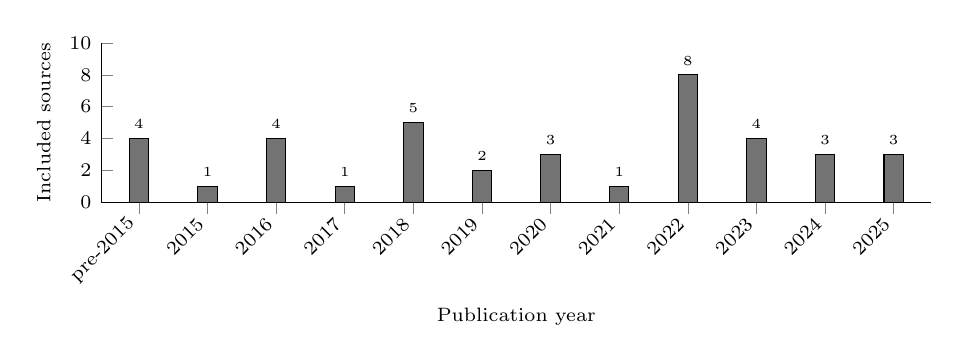
\begin{tikzpicture}
\begin{axis}[
  ybar, width=\columnwidth, height=3.6cm, bar width=7pt,
  ymin=0, ymax=10, ytick={0,2,4,6,8,10}, axis lines*=left,
  symbolic x coords={pre-2015,2015,2016,2017,2018,2019,2020,2021,2022,2023,2024,2025},
  xtick=data, enlarge x limits=0.05,
  x tick label style={rotate=45, anchor=east, font=\scriptsize},
  y tick label style={font=\scriptsize}, label style={font=\scriptsize},
  ylabel={Included sources}, xlabel={Publication year},
  nodes near coords, every node near coord/.append style={font=\tiny},
]
\addplot[fill=black!55, draw=black] coordinates {
  (pre-2015,4) (2015,1) (2016,4) (2017,1) (2018,5) (2019,2)
  (2020,3) (2021,1) (2022,8) (2023,4) (2024,3) (2025,3)};
\end{axis}
\end{tikzpicture}
\caption{Publication year of the 39 sources included in this review (foundational works before 2015 are grouped).}
\label{fig:years}
\end{figure}

%=====================================================================
\section{Background and Technical Foundations}
%=====================================================================
\subsection{Detection Paradigms}
Signature-based detection matches known indicators such as byte patterns or hashes; it is precise for known threats and blind to new ones. Rule-based detection generalises signatures into behavioural conditions, for instance a process connecting to a known backdoor port, and remains transparent because each alert maps to a rule. Supervised ML learns a decision boundary from labelled events or traffic and can model complex patterns, but it depends on representative labels. Unsupervised anomaly detection models normal behaviour and flags deviations, which suits unknown attacks yet produces outliers that are not necessarily malicious~\cite{sommer2010outside}. Deep and hybrid models combine these ideas, for example deep autoencoders feeding a classifier~\cite{shone2018deep}. Table~\ref{tab:approaches} and Fig.~\ref{fig:taxonomy} summarise the paradigms.

\begin{figure}[t]
\centering
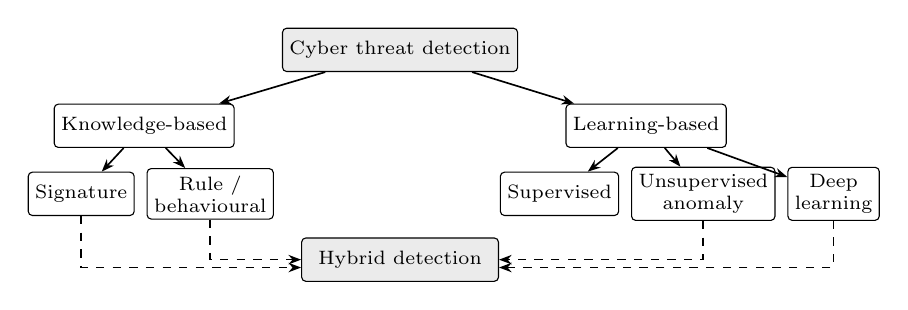
\begin{tikzpicture}[node distance=3mm and 2mm]
\node[box, fill=black!8] (root) {Cyber threat detection};
\node[box, below left=4mm and 6mm of root] (kb) {Knowledge-based};
\node[box, below right=4mm and 6mm of root] (ml) {Learning-based};
\node[box, below=3mm of kb, xshift=-8mm] (sig) {Signature};
\node[box, right=1.5mm of sig] (rule) {Rule /\\behavioural};
\node[box, below=3mm of ml, xshift=-11mm] (sup) {Supervised};
\node[box, right=1.5mm of sup] (uns) {Unsupervised\\anomaly};
\node[box, right=1.5mm of uns] (deep) {Deep\\learning};
\node[box, below=9mm of root, minimum width=25mm, yshift=-12mm, fill=black!8] (hyb) {Hybrid detection};
\draw[arr] (root) -- (kb); \draw[arr] (root) -- (ml);
\draw[arr] (kb) -- (sig); \draw[arr] (kb) -- (rule);
\draw[arr] (ml) -- (sup); \draw[arr] (ml) -- (uns); \draw[arr] (ml) -- (deep);
\draw[arr, dashed] (rule.south) |- (hyb.west);
\draw[arr, dashed] (uns.south) |- (hyb.east);
\draw[arr, dashed] (sig.south) |- ([yshift=-1mm]hyb.west);
\draw[arr, dashed] (deep.south) |- ([yshift=-1mm]hyb.east);
\end{tikzpicture}
\caption{Taxonomy of detection methods. Dashed arrows show that hybrid systems combine knowledge-based and learning-based detectors.}
\label{fig:taxonomy}
\end{figure}

\begin{table*}[t]
\caption{Comparison of Detection Approaches}
\label{tab:approaches}
\centering
\footnotesize
\begin{tabularx}{\textwidth}{@{}p{2.2cm}YYYYp{2.1cm}@{}}
\toprule
\textbf{Approach} & \textbf{Detection principle} & \textbf{Data requirements} & \textbf{Strengths} & \textbf{Limitations} & \textbf{Explainability} \\
\midrule
Signature-based & Match known indicators (patterns, hashes) & Curated signature database & Very low false positives for known threats & Misses new or modified threats; constant updates needed & High (matched indicator) \\
Rule-based & Expert conditions on events or behaviour & Event telemetry; expert knowledge & Transparent; easy to audit and tune & Brittle to evasion; rule maintenance; limited coverage & High (fired rule) \\
Supervised ML & Learn boundary between labelled classes & Large, representative labelled data~\cite{buczak2016survey} & High benchmark accuracy; multi-class labels & Label noise, sampling bias and leakage~\cite{arp2022dos,engelen2021troubleshooting} & Low--medium; needs post-hoc XAI \\
Unsupervised anomaly & Model normality; flag deviations~\cite{liu2008isolation} & Mostly benign data; no labels & Can surface unknown attacks & Outlier $\neq$ attack; high base-rate false alarms~\cite{sommer2010outside} & Low; deviating features can be reported \\
Deep learning & Learn representations from raw or flow data~\cite{shone2018deep,mirsky2018kitsune} & Large data; compute & Models complex patterns; online variants exist~\cite{mirsky2018kitsune} & Opaque; adversarial fragility~\cite{biggio2018wild} & Low; explanation reliability varies~\cite{warnecke2020evaluating} \\
Hybrid & Combine detectors and correlate outputs & Union of the above & Covers each other's blind spots & Integration and calibration complexity & Depends on design \\
\bottomrule
\end{tabularx}
\end{table*}

\subsection{Isolation Forest}
Isolation Forest isolates points with random axis-parallel splits; anomalies need fewer splits than normal points~\cite{liu2008isolation}. For a point $x$ in a sample of size $n$, the anomaly score is
\begin{equation}
s(x,n)=2^{-\mathbb{E}[h(x)]/c(n)},\quad c(n)=2H(n-1)-\frac{2(n-1)}{n},
\label{eq:iforest}
\end{equation}
where $h(x)$ is the path length of $x$ in a tree, $\mathbb{E}[h(x)]$ is its mean over the forest, $c(n)$ is the average path length of an unsuccessful binary-search-tree lookup used for normalisation, and $H(i)\approx\ln i+0.5772$. Scores from \eqref{eq:iforest} that approach 1 indicate anomalies. Sub-sampling gives linear time and low memory~\cite{liu2008isolation}, which explains its use as a baseline in online detectors~\cite{mirsky2018kitsune} and in alert prioritisation~\cite{aminanto2020threat}. Its weaknesses are equally relevant: the score is relative to the training sample, the method assumes anomalies are few and different, and it cannot express \emph{why} a point is unusual without additional analysis.

\subsection{Evaluation Metrics}
With true and false positives and negatives $TP, FP, TN, FN$, precision $P=TP/(TP+FP)$, recall $R=TP/(TP+FN)$, false-positive rate $\mathit{FPR}=FP/(FP+TN)$ and
\begin{equation}
F_1=\frac{2PR}{P+R}.
\label{eq:f1}
\end{equation}
Although \eqref{eq:f1} balances precision and recall, it does not show the alarm volume: when benign traffic dominates, a small $\mathit{FPR}$ still yields many false alarms, which is the base-rate problem highlighted for security ML~\cite{arp2022dos}. Averaged scores weighted by class support can also hide failure on minority classes; we return to this in Section~IV-B.

\subsection{Explainability, Risk and Human Oversight}
Post-hoc explainers such as LIME fit a local surrogate around one prediction~\cite{ribeiro2016why}, and SHAP attributes a prediction to features using Shapley values~\cite{lundberg2017unified}. Risk assessment ranks alerts by likely impact rather than by detector confidence alone, and countermeasure-selection research studies how to choose a response once risk is known~\cite{nespoli2018optimal}. Human-in-the-loop response keeps a person responsible for actions that can disrupt users. RAG grounds an LLM's output in retrieved documents~\cite{lewis2020retrieval}, which is attractive for producing alert explanations from organisational knowledge.

%=====================================================================
\section{Literature Review and Comparative Analysis}
%=====================================================================
\subsection{Detection Methods and Reported Performance}
Table~\ref{tab:studies} lists representative studies. Older benchmarks are still used for headline numbers. Shone et al.\ evaluated a stacked non-symmetric deep autoencoder on KDD Cup~99 and NSL-KDD and reported 97.85\% accuracy for five-class KDD classification, but 85.42\% on five-class NSL-KDD~\cite{shone2018deep}. The drop is telling, since NSL-KDD was built to remove the duplicate records that inflate KDD results~\cite{tavallaee2009detailed}. Some recent conference papers also report accuracy without naming the dataset or protocol; one reports 93\% and 96\% accuracy for CNN and RNN models on unnamed ``real-world vulnerability datasets''~\cite{rajendran2024cybersecurity}, and another demonstrates graph neural networks with LIME and an LLM for interpretation without reporting quantitative results~\cite{balaji2025explainable}. Such results cannot be compared with the benchmark literature.

Online, resource-constrained detection is a distinct line of work. Kitsune trains an ensemble of small autoencoders incrementally and runs on a Raspberry Pi; its authors report detection close to offline Gaussian mixture and Isolation Forest baselines and a better equal error rate than the batch Gaussian mixture model on six of its attack datasets~\cite{mirsky2018kitsune}. Isolation Forest also appears in alert triage: Aminanto et al.\ combine it with a stacked autoencoder to prioritise SOC alerts and use day-forward chaining so that evaluation respects time order~\cite{aminanto2020threat}. Provenance-based triage takes a different route, scoring alerts by the rarity of the causal paths that led to them~\cite{hassan2019nodoze}. On RQ2, these studies point the same way. Isolation Forest is attractive because it is fast and needs no labels, and it seems most useful as one signal in a larger triage process instead of a detector on its own.

\begin{table*}[t]
\caption{Comparison of Published Studies (results as reported by the authors; not directly comparable across rows)}
\label{tab:studies}
\centering
\footnotesize
\begin{tabularx}{\textwidth}{@{}p{1.75cm}p{2.5cm}YYp{1.7cm}Yp{3.0cm}@{}}
\toprule
\textbf{Ref. (year)} & \textbf{Objective} & \textbf{Method} & \textbf{Dataset} & \textbf{Metrics} & \textbf{Reported results} & \textbf{Limitations} \\
\midrule
\cite{shone2018deep} (2018) & Reduce human effort and improve NIDS accuracy & Stacked non-symmetric deep autoencoders + random forest & KDD Cup 99; NSL-KDD & Accuracy, precision, recall, F-score & 97.85\% (KDD, 5-class); 85.42\% (NSL-KDD, 5-class); 89.22\% (13-class) & KDD duplicates~\cite{tavallaee2009detailed}; weak minority classes \\
\cite{mirsky2018kitsune} (2018) & Lightweight online NIDS & Ensemble of incremental autoencoders (KitNET) & IP camera surveillance and IoT network captures & AUC, EER, TPR at fixed FPR & Close to offline GMM/iForest; better EER than GMM on six attack datasets & Unsupervised alarms unlabelled by type; per-network training \\
\cite{aminanto2020threat} (2020) & Prioritise SOC threat alerts & Isolation Forest + stacked autoencoder, day-forward chaining & Enterprise alert logs & Not reported here & Not reported here (qualitative use only) & Results tied to one organisation's alerts \\
\cite{engelen2021troubleshooting} (2021) & Audit benchmark quality & Re-examined generation, flow construction, features, labels & CICIDS2017 & Benchmark re-runs & $>$20\% of traces reconstructed or relabelled & Focused on one dataset \\
\cite{sarhan2022standard} (2022) & Common feature set across datasets & NetFlow v9 features (43) + Extra Trees & UNSW-NB15, BoT-IoT, ToN-IoT, CSE-CIC-IDS2018 & Accuracy, AUC, F1, DR, FAR & Binary F1 0.97 (NF-UNSW-NB15-v2) vs 0.92 (original); see Fig.~\ref{fig:featuresets} & Within-dataset splits only \\
\cite{rajendran2024cybersecurity} (2024) & Unified DL and anomaly-based detection & CNN, RNN with anomaly detection & ``Real-world vulnerability datasets'' (unnamed) & Accuracy, FPR & CNN 93\%, RNN 96\% accuracy; FPR 5\% & Dataset and protocol not specified \\
\cite{balaji2025explainable} (2025) & Interpretable threat detection & GCN + LIME + LLM explanations & ``Cybersecurity dataset'' (unnamed) & Not reported & Not reported (qualitative explanations) & No quantitative evaluation \\
\cite{liu2025cylens} (2025, preprint) & LLM support across CTI lifecycle & LLM with knowledge from 271,570 threat reports and six NLP modules & Threat reports, CVE/NVD & Task-specific & Reported to outperform leading LLMs and security agents (authors' claim) & Preprint; LLM security risks~\cite{greshake2023indirect} \\
\bottomrule
\end{tabularx}
\end{table*}

\subsection{Datasets and Evaluation Validity}
Most quantitative evidence on ML-based threat detection comes from network intrusion benchmarks, so their quality shapes what the field believes about detection performance. Dataset defects are the best-documented problem here (RQ7). In KDD Cup~99, about 78\% of training and 75\% of test records are duplicates~\cite{tavallaee2009detailed}. UNSW-NB15 was introduced to provide modern traffic and nine attack families~\cite{moustafa2015unsw}, and CICIDS2017 to provide realistic benign profiles and current attacks~\cite{sharafaldin2018toward}; yet a later audit of CICIDS2017 reconstructed or relabelled more than 20\% of its traffic traces and showed that benchmark results changed as a consequence~\cite{engelen2021troubleshooting}. Table~\ref{tab:datasets} compares the three datasets.

Feature representation matters as much as data quality. Sarhan et al.\ extracted the same NetFlow features from several datasets and evaluated one classifier with one protocol~\cite{sarhan2022standard}. Their results, re-plotted in Fig.~\ref{fig:featuresets}, show that the choice of feature set alone moves binary F1 on CSE-CIC-IDS2018 from 0.83 to 0.97 and the false alarm rate from 4.59\% to 0.31\%. Because the classifier and protocol are fixed, the differences come from representation, not from algorithm quality. The same study shows how class imbalance hides failure. On UNSW-NB15, the weighted multi-class F1 was 0.98, but per-class F1 was 0.03 for \textit{Analysis}, 0.08 for \textit{Backdoor} and 0.09 for \textit{Worms}~\cite{sarhan2022standard}, classes that make up 2,677, 2,329 and 174 of the 2,540,044 records~\cite{moustafa2015unsw}. Fig.~\ref{fig:imbalance} relates frequency to per-class F1. A simple imbalance ratio,
\begin{equation}
\rho=\frac{\max_k N_k}{\min_k N_k},
\label{eq:imbalance}
\end{equation}
where $N_k$ is the number of records of class $k$. For UNSW-NB15, \eqref{eq:imbalance} gives $2{,}218{,}761/174\approx1.3\times10^4$. With imbalance of this size, weighted averages mainly reflect the majority classes.

\begin{figure}[t]
\centering
% Data: paper/data/fig2_feature_sets_f1.csv (Table 8 of Sarhan et al.).
\pgfplotsset{fsets/.style={
  ybar, width=\columnwidth, bar width=5pt, axis lines*=left,
  symbolic x coords={UNSW-NB15,BoT-IoT,ToN-IoT,CSE-CIC-IDS2018},
  xtick=data, enlarge x limits=0.15,
  tick label style={font=\scriptsize}, label style={font=\scriptsize}}}
\begin{tikzpicture}
\begin{axis}[fsets, height=3.4cm, ymin=0.75, ymax=1.02, ylabel={F1-score},
  xticklabel=\empty,
  legend style={at={(0.5,1.04)}, anchor=south, legend columns=3, draw=none, font=\scriptsize,
    /tikz/every even column/.append style={column sep=3mm}}]
\addplot[fill=black!15, draw=black] coordinates {(UNSW-NB15,0.92) (BoT-IoT,1.00) (ToN-IoT,0.99) (CSE-CIC-IDS2018,0.94)};
\addplot[fill=black!50, draw=black] coordinates {(UNSW-NB15,0.85) (BoT-IoT,0.97) (ToN-IoT,1.00) (CSE-CIC-IDS2018,0.83)};
\addplot[fill=black!90, draw=black] coordinates {(UNSW-NB15,0.97) (BoT-IoT,1.00) (ToN-IoT,1.00) (CSE-CIC-IDS2018,0.97)};
\legend{Original features, NetFlow basic, NetFlow extended}
\end{axis}
\end{tikzpicture}\\[1mm]
\begin{tikzpicture}
\begin{axis}[fsets, height=3.4cm, ymin=0, ymax=5, ylabel={False alarm rate (\%)}]
\addplot[fill=black!15, draw=black] coordinates {(UNSW-NB15,0.35) (BoT-IoT,1.05) (ToN-IoT,2.10) (CSE-CIC-IDS2018,1.07)};
\addplot[fill=black!50, draw=black] coordinates {(UNSW-NB15,1.01) (BoT-IoT,1.13) (ToN-IoT,0.37) (CSE-CIC-IDS2018,4.59)};
\addplot[fill=black!90, draw=black] coordinates {(UNSW-NB15,0.16) (BoT-IoT,0.26) (ToN-IoT,0.58) (CSE-CIC-IDS2018,0.31)};
\end{axis}
\end{tikzpicture}
\caption{Binary F1 and false alarm rate of one Extra Trees classifier under three feature sets (same protocol: 70/30 split, mean of five splits). Data from Table~8 of~\cite{sarhan2022standard}.}
\label{fig:featuresets}
\end{figure}

\begin{figure}[t]
\centering
% Data: paper/data/fig3_unsw_nb15_classes.csv (Moustafa & Slay Table VIII; Sarhan et al. Table 9).
% scale only axis: both overlaid axes get the same plot area, and the left and right
% labels sit outside it, so the figure stays within the column.
\pgfplotsset{unswx/.style={
  scale only axis, width=0.68\columnwidth, height=3.1cm, enlarge x limits=0.06,
  symbolic x coords={Normal,Generic,Exploits,Fuzzers,DoS,Reconnaissance,Analysis,Backdoor,Shellcode,Worms},
  xtick=data, tick label style={font=\scriptsize}, label style={font=\scriptsize}}}
\begin{tikzpicture}
\begin{axis}[unswx, ybar, bar width=8pt, ymode=log, log origin=infty,
  ymin=100, ymax=1e7, axis y line*=left, axis x line*=bottom,
  ylabel={Records in data set (log scale)},
  x tick label style={rotate=45, anchor=east}]
\addplot[fill=black!15, draw=black] coordinates {
  (Normal,2218761) (Generic,215481) (Exploits,44525) (Fuzzers,24246) (DoS,16353)
  (Reconnaissance,13987) (Analysis,2677) (Backdoor,2329) (Shellcode,1511) (Worms,174)};
\end{axis}
\begin{axis}[unswx, ymin=0, ymax=1.12, axis y line*=right, axis x line=none, ytick={0,0.5,1},
  ylabel={Per-class F1-score}]
\addplot[black, thick, mark=*, mark size=1.3pt] coordinates {
  (Normal,1.00) (Generic,0.91) (Exploits,0.80) (Fuzzers,0.57) (DoS,0.18)
  (Reconnaissance,0.80) (Analysis,0.03) (Backdoor,0.08) (Shellcode,0.59) (Worms,0.09)};
\draw[dashed] (rel axis cs:0,0.875) -- (rel axis cs:1,0.875); % 0.98 / 1.12
\node[font=\tiny, anchor=south east, inner sep=1pt] at (rel axis cs:1,0.885) {weighted F1 = 0.98};
\end{axis}
\end{tikzpicture}
\caption{UNSW-NB15 class frequency (bars, log scale; from~\cite{moustafa2015unsw}) and per-class F1 of an Extra Trees model on the original features (line; from~\cite{sarhan2022standard}). The two series come from different papers and are combined only to relate frequency to detection quality.}
\label{fig:imbalance}
\end{figure}

Methodological critiques reach similar conclusions from other directions. Arp et al.\ identify ten pitfalls, including sampling bias, data snooping and inappropriate baselines, and find them in a sample of 30 top-tier papers~\cite{arp2022dos}. TESSERACT shows that ignoring time when splitting malware data inflates results and proposes temporally consistent evaluation~\cite{pendlebury2019tesseract}. Kapoor and Narayanan document data leakage across 17 fields and 294 papers and propose a taxonomy of eight leakage types~\cite{kapoor2023leakage}. For RQ8, the evidence supports three practices: use a common feature schema before comparing datasets~\cite{sarhan2022standard}; train on one dataset and test on another, reporting the drop
\begin{equation}
\Delta F_1 = F_1^{\,\mathrm{in}} - F_1^{\,\mathrm{cross}},
\label{eq:shift}
\end{equation}
where $F_1^{\,\mathrm{in}}$ is measured on a held-out split of the training dataset and $F_1^{\,\mathrm{cross}}$ on a different dataset; and use explanations to check whether the model relies on the same features in both domains, as Layeghy and Portmann do in their cross-domain analysis~\cite{layeghy2023explainable}. Datasets with different native feature schemas, such as KDD Cup~99's 41 connection features and UNSW-NB15's 49 Argus/Bro features, should not be merged column by column, because identically named or similar fields are computed differently and the merged data would mix incompatible distributions.

\begin{table}[t]
\caption{Comparison of Network Intrusion Detection Benchmark Datasets}
\label{tab:datasets}
\centering
\footnotesize
\setlength{\tabcolsep}{2.5pt}
\begin{tabularx}{\columnwidth}{@{}p{1.25cm}YYY@{}}
\toprule
 & \textbf{KDD Cup 99} & \textbf{UNSW-NB15} & \textbf{CICIDS2017} \\
\midrule
Origin & DARPA'98 simulated military network~\cite{tavallaee2009detailed} & IXIA PerfectStorm testbed, 2015~\cite{moustafa2015unsw} & CIC testbed with profiled benign users~\cite{sharafaldin2018toward} \\
Attacks & DoS, Probe, R2L, U2R & Nine families (e.g., Fuzzers, Exploits, Generic, Worms) & Benign plus seven common attack types (e.g., DoS, brute force, web, botnet) \\
Features & 41 per connection & 49 (Argus, Bro and derived) & Flow features (CICFlowMeter) \\
Strengths & Long history; many baselines & Modern low-footprint attacks; labelled families & Realistic benign traffic; recent attacks \\
Limitations & $\approx$78\%/75\% duplicate train/test records~\cite{tavallaee2009detailed}; dated traffic & Strong class imbalance (Fig.~\ref{fig:imbalance}) & $>$20\% traces needed reconstruction or relabelling~\cite{engelen2021troubleshooting} \\
Suitability & Historical comparison only (prefer NSL-KDD) & Multi-class studies with per-class reporting & Use corrected versions; temporal splits \\
\bottomrule
\end{tabularx}
\end{table}

\subsection{Behavioural Ransomware Detection}
Ransomware detection research has converged on behavioural signals from the file system (RQ6). CryptoDrop combines indicators such as changes in file type, loss of similarity between file versions and high output entropy, raising an alert when several occur together~\cite{scaife2016cryptolock}. ShieldFS builds models of normal filesystem activity from a study of benign applications and, when a process deviates, reverts its changes through a copy-on-write layer~\cite{continella2016shieldfs}. Later surveys organise this space: Oz et al.\ review 137 studies from 1990 to 2020 across PCs, mobile and IoT~\cite{oz2022survey}, and Urooj et al.\ focus on dynamic analysis with ML between 2019 and 2021~\cite{urooj2022ransomware}. The recurring difficulty is that backup, synchronisation, compression and build tools also rewrite many files quickly. The literature handles this in two ways, by correlating several weak indicators and by tying activity to a responsible process so that a response can be targeted. Attribution is reliable when detection happens in the file-system driver, as in ShieldFS, and much harder for user-mode monitors that observe file events without process identity.

\subsection{Explainability for Security Alerts}
XAI work in security has moved from applying generic explainers to asking whether explanations are fit for purpose (RQ3). Warnecke et al.\ propose general and security-specific criteria and show that popular explanation methods differ considerably when applied to security models~\cite{warnecke2020evaluating}. Nadeem et al.\ systematise XAI for security, including the risk that explanations can be used offensively~\cite{nadeem2023sok}, and Neupane et al.\ survey explainable IDS, discussing the trade-off between performance and explainability and proposing a human-in-the-loop architecture~\cite{neupane2022xids}. The analyst perspective adds a different requirement: SOC practitioners asked for alarms that are reliable, explainable, analytical, contextual and transferable, and they noted that most false positives were benign triggers caused by legitimate behaviour~\cite{alahmadi2022false}. Explanations that list feature attributions therefore answer only part of the analyst's question. They need to be combined with context about the asset and the organisation.

\subsection{Contextual Risk and Alert Prioritisation}
Context changes the value of an alert (RQ4). Alarm fatigue is driven less by missed attacks than by benign alerts that lack context~\cite{alahmadi2022false}, and prioritisation methods based on anomaly scores~\cite{aminanto2020threat} or provenance~\cite{hassan2019nodoze} reduce the analyst's load by ranking rather than filtering. Countermeasure-selection frameworks add cost and impact models to choose responses~\cite{nespoli2018optimal}, and dashboard studies with emergency response teams show that analysts value aggregated, filterable situational information~\cite{kaufhold2022cyber}. We found few evaluations that test whether a particular contextual weighting ranks alerts better than detector scores alone.

\subsection{Automation, Human Oversight and Accountability}
Studies of SOC automation describe a spectrum rather than a binary choice (RQ5). Tilbury and Flowerday screened 599 articles, retained 49, and proposed a matrix of four human--automation combinations~\cite{tilbury2024humans}. Full automation reduces response time but turns the response mechanism into an attack surface; adversarial ML research shows that learned components can be manipulated~\cite{biggio2018wild}, and a manipulated detector that can terminate processes is more dangerous than one that only raises alerts. Human approval adds latency and depends on the quality of the evidence presented. Accountability has older roots: Schneier and Kelsey proposed cryptographic audit logs whose entries cannot be read or altered undetectably after a compromise~\cite{schneier1999secure}, yet response frameworks rarely report how their decisions are logged or audited.

\subsection{LLMs and Retrieval-Augmented Assistance}
LLM research in security is growing quickly; one systematic review analyses 185 papers in its latest preprint version~\cite{xu2024llm}. CyLens, also a preprint, integrates knowledge from 271,570 threat reports to support attribution, prioritisation and remediation~\cite{liu2025cylens}. RAG can ground explanations in vetted documents~\cite{lewis2020retrieval}, but it also creates a channel for indirect prompt injection, in which instructions hidden in retrieved content take control of the model~\cite{greshake2023indirect}. For RQ9 the evidence suggests that LLMs are promising for explanation and summarisation, provided that they are kept away from executing actions, that retrieved text is treated as untrusted data, and that answers separate evidence from recommendation. We found no controlled study showing that LLM explanations improve analysts' decisions on real alerts.

%=====================================================================
\section{Research Gaps and Open Challenges}
%=====================================================================
Table~\ref{tab:gaps} assesses the seven preliminary gaps against the evidence (RQ10). Two of them, G1 (evaluation validity) and G7 (accountability), are well established as problems; G1 is also partly addressed by published remedies, so a new evaluation pipeline alone would not be a novel contribution. G5 (explainability) is extensively studied as a method problem, but rarely as a decision-support problem. G2 (detection without response) and G6 (unsafe automation) are discussed in reaction-framework and SOC-automation research, yet these lines seldom connect to detection and explanation in a single evaluated system. G3 (adaptivity) remains open where it matters most, namely drift detection and retraining under realistic time order~\cite{pendlebury2019tesseract}. G4 (risk context) is supported by analyst studies but lacks empirical evidence that particular weightings help.

Fig.~\ref{fig:results} brings together the reported results that motivate G1. For each case it pairs a study's headline figure with the same study's result under a stricter view: a de-duplicated benchmark~\cite{shone2018deep,tavallaee2009detailed}, the weakest attack class instead of the support-weighted average, or the least favourable of three feature sets~\cite{sarhan2022standard}. The stricter value is lower in every case, by between 12 and 95 percentage points. No row compares one study with another; each shows how much a single reported number depends on choices that papers do not always make visible.

\begin{figure}[t]
\centering
% Data: paper/data/fig_results_comparison.csv
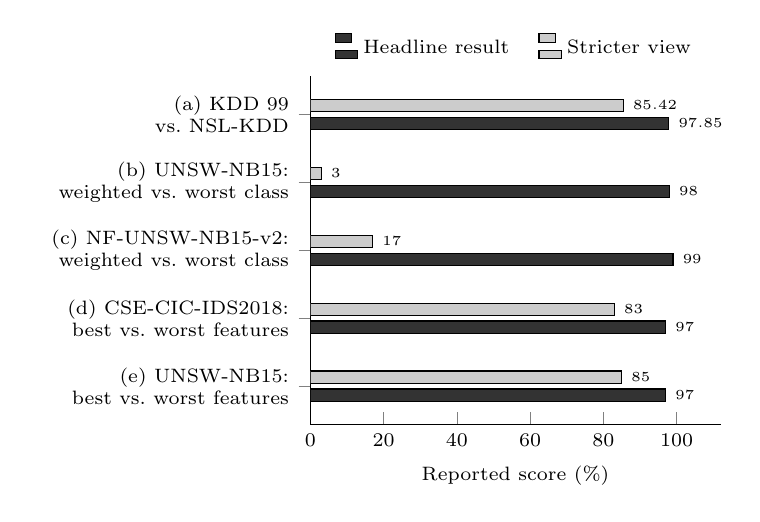
\begin{tikzpicture}
\begin{axis}[
  xbar, width=0.56\columnwidth, height=6cm, bar width=4.5pt,
  xmin=0, xmax=112, axis lines*=left, y dir=reverse,
  symbolic y coords={shone,unsworig,unswnf,cicfs,unswfs}, ytick=data,
  yticklabels={{(a) KDD 99 vs.\ NSL-KDD},
               {(b) UNSW-NB15:\\weighted vs.\ worst class},
               {(c) \mbox{NF-UNSW-NB15-v2}:\\weighted vs.\ worst class},
               {(d) \mbox{CSE-CIC-IDS2018}:\\best vs.\ worst features},
               {(e) UNSW-NB15:\\best vs.\ worst features}},
  yticklabel style={font=\scriptsize, align=right, text width=3.2cm},
  xticklabel style={font=\scriptsize}, label style={font=\scriptsize},
  xlabel={Reported score (\%)}, enlarge y limits=0.14,
  nodes near coords, every node near coord/.append style={font=\tiny},
  legend style={at={(0.5,1.02)}, anchor=south, legend columns=2, draw=none, font=\scriptsize,
    /tikz/every even column/.append style={column sep=3mm}},
]
\addplot[fill=black!80, draw=black] coordinates {(97.85,shone) (98,unsworig) (99,unswnf) (97,cicfs) (97,unswfs)};
\addplot[fill=black!20, draw=black] coordinates {(85.42,shone) (3,unsworig) (17,unswnf) (83,cicfs) (85,unswfs)};
\legend{Headline result, Stricter view}
\end{axis}
\end{tikzpicture}
\caption{Headline results versus the same study's result under a stricter view: (a) five-class accuracy of one model on KDD Cup~99 and on de-duplicated NSL-KDD~\cite{shone2018deep}; (b), (c) support-weighted versus lowest per-class F1; (d), (e) binary F1 of the best versus the worst of three feature sets~\cite{sarhan2022standard}. Rows are not comparable with each other.}
\label{fig:results}
\end{figure}

\begin{figure*}[t]
\centering
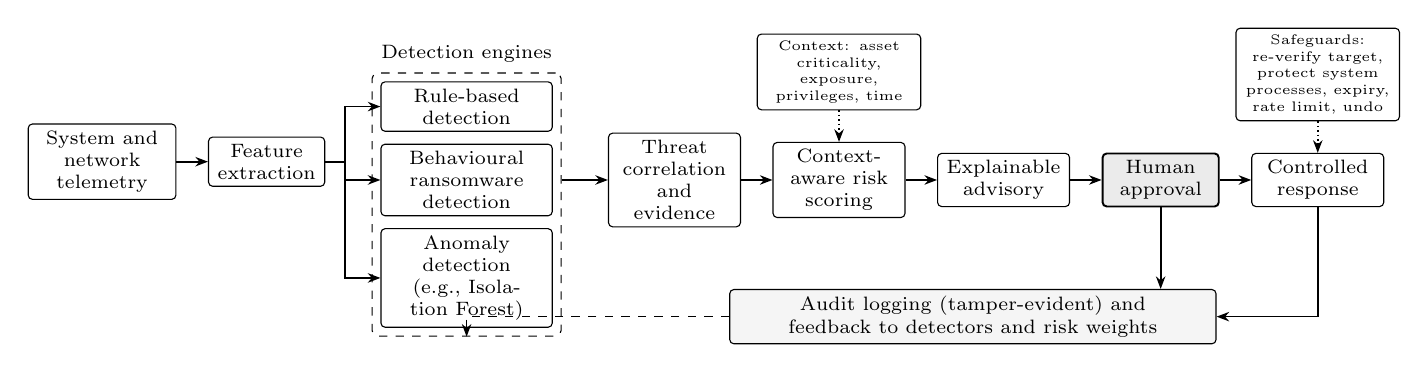
\begin{tikzpicture}[node distance=4mm]
\node[box, text width=17mm] (tel) {System and network telemetry};
\node[box, right=of tel, text width=13mm] (fe) {Feature extraction};
\node[box, right=7mm of fe, yshift=7mm, text width=20mm] (rule) {Rule-based detection};
\node[box, below=1.5mm of rule, text width=20mm] (rans) {Behavioural ransomware detection};
\node[box, below=1.5mm of rans, text width=20mm] (anom) {Anomaly detection (e.g., Isolation Forest)};
\node[grp, fit=(rule)(rans)(anom), label={[font=\scriptsize]above:Detection engines}] (det) {};
\node[box, right=7mm of rans, text width=15mm] (corr) {Threat correlation and evidence};
\node[box, right=of corr, text width=15mm] (risk) {Context-aware risk scoring};
\node[box, right=of risk, text width=15mm] (adv) {Explainable advisory};
\node[human, right=of adv, text width=13mm] (hum) {Human approval};
\node[box, right=of hum, text width=15mm] (resp) {Controlled response};
\node[box, below=9mm of risk, text width=60mm, xshift=17mm, fill=black!4] (audit) {Audit logging (tamper-evident) and feedback to detectors and risk weights};
\node[box, above=4mm of resp, text width=19mm, font=\tiny] (safe) {Safeguards: re-verify target, protect system processes, expiry, rate limit, undo};
\node[box, above=4mm of risk, text width=19mm, font=\tiny] (ctx) {Context: asset criticality, exposure, privileges, time};
\draw[arr] (tel) -- (fe);
\draw[arr] (fe.east) -- ++(2.5mm,0) |- (rule.west);
\draw[arr] (fe.east) -- ++(2.5mm,0) |- (rans.west);
\draw[arr] (fe.east) -- ++(2.5mm,0) |- (anom.west);
\draw[arr] (det.east |- corr) -- (corr);
\draw[arr] (corr) -- (risk); \draw[arr] (risk) -- (adv); \draw[arr] (adv) -- (hum); \draw[arr] (hum) -- (resp);
\draw[arr, densely dotted] (ctx) -- (risk);
\draw[arr, densely dotted] (safe) -- (resp);
\draw[arr] (resp.south) |- (audit.east);
\draw[arr] (hum.south) -- (hum.south |- audit.north);
\draw[arr, dashed] (audit.west) -| (det.south);
\end{tikzpicture}
\caption{Proposed conceptual framework for explainable, risk-aware threat detection with human-approved response. It is derived from the reviewed literature and has not been experimentally validated.}
\label{fig:framework}
\end{figure*}

\begin{figure}[t]
\centering
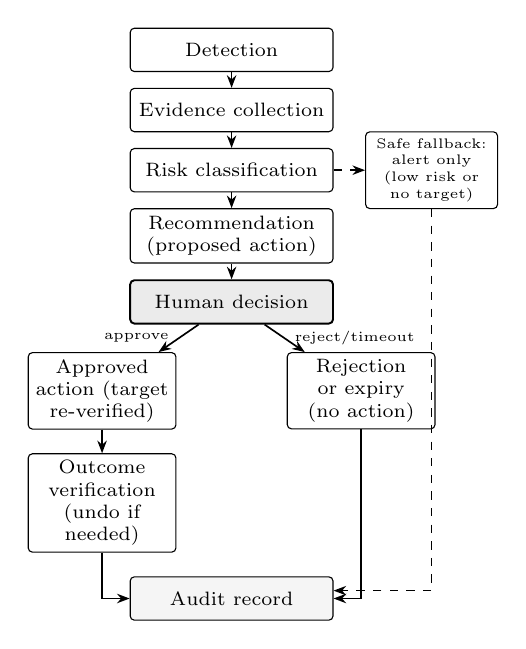
\begin{tikzpicture}[node distance=2mm]
\node[box, text width=24mm] (d) {Detection};
\node[box, below=of d, text width=24mm] (e) {Evidence collection};
\node[box, below=of e, text width=24mm] (r) {Risk classification};
\node[box, below=of r, text width=24mm] (rec) {Recommendation (proposed action)};
\node[human, below=of rec, text width=24mm] (h) {Human decision};
\node[box, below left=3.5mm and -6mm of h, text width=17mm] (ap) {Approved action (target re-verified)};
\node[box, below right=3.5mm and -6mm of h, text width=17mm] (rej) {Rejection or expiry (no action)};
\node[box, below=3mm of ap, text width=17mm] (ver) {Outcome verification (undo if needed)};
\node[box, text width=24mm, fill=black!4, anchor=north] (au) at ([yshift=-3mm]h |- ver.south) {Audit record};
\node[box, right=4mm of r, text width=15mm, font=\tiny] (fb) {Safe fallback: alert only (low risk or no target)};
\draw[arr] (d) -- (e); \draw[arr] (e) -- (r); \draw[arr] (r) -- (rec); \draw[arr] (rec) -- (h);
\draw[arr] (h) -- node[left, font=\tiny] {approve} (ap);
\draw[arr] (h) -- node[right, font=\tiny] {reject/timeout} (rej);
\draw[arr] (ap) -- (ver);
\draw[arr] (ver.south) |- (au.west);
\draw[arr] (rej.south) |- (au.east);
\draw[arr, dashed] (r) -- (fb);
\draw[arr, dashed] (fb.south) |- ([yshift=1mm]au.east);
\end{tikzpicture}
\caption{Human-in-the-loop response workflow with safe fallback, rejection and expiry paths.}
\label{fig:hitl}
\end{figure}

\begin{table*}[t]
\caption{Research Gaps and Opportunities (status assessed from the reviewed evidence)}
\label{tab:gaps}
\centering
\footnotesize
\begin{tabularx}{\textwidth}{@{}p{1.55cm}p{2.0cm}YYYY@{}}
\toprule
\textbf{Gap (status)} & \textbf{Supporting literature} & \textbf{Identified limitation} & \textbf{Research significance} & \textbf{Proposed direction} & \textbf{Suggested evaluation} \\
\midrule
G1 Evaluation validity (established; partly addressed) & \cite{tavallaee2009detailed,engelen2021troubleshooting,arp2022dos,kapoor2023leakage,pendlebury2019tesseract} & Duplicates, label errors, leakage and random splits inflate scores & Reported gains may not transfer to deployment & Corrected data, temporal splits, common feature schema & Cross-dataset $\Delta F_1$ (Eq.~\ref{eq:shift}); per-class F1 \\
G2 Detection without response (partly addressed) & \cite{nespoli2018optimal,tilbury2024humans} & Response studied apart from detection & Alerts without actionable next steps & Link detections to graded, policy-bound responses & Time to containment; decision accuracy in user studies \\
G3 Weak adaptivity (open) & \cite{pendlebury2019tesseract,mirsky2018kitsune,layeghy2023explainable} & Few systems detect drift or retrain safely & Performance decays as behaviour changes & Drift monitoring with controlled retraining & Rolling time-ordered evaluation \\
G4 Missing risk context (open) & \cite{alahmadi2022false,aminanto2020threat,kaufhold2022cyber} & Context rarely modelled or validated & Benign triggers dominate analyst load & Asset- and exposure-aware scoring & Ranking quality (e.g., precision at top-$k$) against analyst labels \\
G5 Poor explainability (partly addressed) & \cite{warnecke2020evaluating,nadeem2023sok,neupane2022xids,ribeiro2016why} & Explanations judged by fidelity, not usefulness & Trust and correct action depend on understanding & Evidence-plus-context explanations; grounded LLM summaries & Analyst studies: accuracy, time, trust calibration \\
G6 Unsafe automatic response (partly addressed) & \cite{biggio2018wild,tilbury2024humans,greshake2023indirect} & Automation can be manipulated or misfire & Response becomes an attack surface & Human approval, target re-verification, expiry, rate limits & Red-team tests of the response path \\
G7 Accountability (established; open in practice) & \cite{schneier1999secure,tilbury2024humans} & Decisions seldom logged verifiably & Post-incident review and liability & Tamper-evident logs of every decision & Tamper-detection tests; audit completeness \\
\bottomrule
\end{tabularx}
\end{table*}

%=====================================================================
\section{Proposed Conceptual Framework and Future Directions}
%=====================================================================
Fig.~\ref{fig:framework} presents a conceptual framework informed by the review. It is a proposal for evaluation, not a validated system. Telemetry from processes, network connections and watched folders is turned into features and passed to three complementary detectors: rules for known behaviour, a behavioural ransomware detector for file-system bursts~\cite{scaife2016cryptolock,continella2016shieldfs}, and an anomaly detector such as Isolation Forest for unknown behaviour~\cite{liu2008isolation}. Correlation merges repeated findings and attaches evidence. Risk is then scored in context. As a proposed formulation, not an established standard,
\begin{equation}
r=\min\!\Big(1,\;\sum_{i} w_i\, s_i \prod_{j} m_j\Big),
\label{eq:risk}
\end{equation}
where $s_i\in[0,1]$ are normalised severity, confidence and impact signals with weights $w_i$ summing to one, and $m_j$ are context multipliers for asset criticality, network exposure or privileged accounts. Each multiplier should be stored with the alert so that the score can be explained. Eq.~\eqref{eq:risk} could be evaluated by comparing the ranking it produces with analyst-assigned priorities, and by ablating each multiplier.

The advisory stage presents evidence, the reasons behind the risk level and recommended steps. If an LLM is used, it should be confined to explanation, with retrieved text marked as untrusted~\cite{greshake2023indirect}. Containment follows the workflow in Fig.~\ref{fig:hitl}: actions are proposed only above a risk threshold and only for an identified target, the target is re-verified at approval time, proposals expire, rejection is a normal outcome, and every decision and outcome is written to a tamper-evident log~\cite{schneier1999secure}.

Several directions follow. Detectors should be evaluated with temporal and cross-dataset protocols and per-class reporting. Contextual risk models need ranking studies against analyst judgements. Explanations should be tested with analysts, measuring decision accuracy, time and trust calibration rather than fidelity alone. Response paths need adversarial testing, because the safeguards in Fig.~\ref{fig:hitl} are only useful if they hold under attack. For ransomware, user-mode monitors need better process attribution, which kernel-level event sources may provide. Finally, LLM assistants should be evaluated for both explanation quality and resistance to prompt injection.

%=====================================================================
\section{Conclusion}
%=====================================================================
The literature we reviewed is strong on detection techniques and weaker on evidence that they hold up in operation. Dataset defects, leakage and class imbalance can shift reported scores by large margins, as Figs.~\ref{fig:featuresets}--\ref{fig:results} show, so a headline accuracy figure says little when comparing systems. Explainability research is moving from method design to fitness for purpose, but analyst-centred evaluation is still rare. Response automation, risk context and accountability are each studied, yet seldom together with detection and explanation. Of the seven preliminary gaps, evaluation validity and accountability are well established, explainability and safe response are partly addressed, and adaptivity and validated risk context remain most open.

This review has limitations. It is a structured narrative review based on a seed set and targeted searches, not an exhaustive systematic review, and screening counts were not recorded. Numerical comparisons were limited to results obtained under a shared protocol, which excluded many studies. The quantitative evidence also comes mainly from network intrusion benchmarks; in the sources we reviewed, host-level threat detection, including ransomware detection, lacked comparable public benchmarks, so conclusions about evaluation transfer to it only partly. The proposed framework and risk formulation have not been validated. Future work should evaluate such integrated designs end to end, with analysts in the loop and under realistic, time-ordered and adversarial conditions.

% BEGIN BIBLIOGRAPHY (generated by scripts/build_bibliography.py)

\begin{thebibliography}{99}

\bibitem{buczak2016survey} A. L.~Buczak and E.~Guven, ``A Survey of Data Mining and Machine Learning Methods for Cyber Security Intrusion Detection,'' \emph{IEEE Communications Surveys \& Tutorials}, vol. 18, no. 2, pp. 1153--1176, 2016, doi: 10.1109/COMST.2015.2494502.

\bibitem{sommer2010outside} R.~Sommer and V.~Paxson, ``Outside the Closed World: On Using Machine Learning for Network Intrusion Detection,'' in \emph{Proc. IEEE Symposium on Security and Privacy}, 2010, pp. 305--316, doi: 10.1109/SP.2010.25.

\bibitem{alahmadi2022false} B. A.~Alahmadi, L.~Axon, and I.~Martinovic, ``99\% False Positives: A Qualitative Study of {SOC} Analysts' Perspectives on Security Alarms,'' in \emph{Proc. 31st USENIX Security Symposium}, 2022.

\bibitem{arp2022dos} D.~Arp \emph{et al.}, ``Dos and Don'ts of Machine Learning in Computer Security,'' in \emph{Proc. 31st USENIX Security Symposium}, 2022, pp. 3971--3988.

\bibitem{apruzzese2022role} G.~Apruzzese \emph{et al.}, ``The Role of Machine Learning in Cybersecurity,'' \emph{Digital Threats: Research and Practice}, 2022, doi: 10.1145/3545574.

\bibitem{schmitt2025cyber} M.~Schmitt and P.~Koutroumpis, ``Cyber Shadows: Neutralizing Security Threats With {AI} and Targeted Policy Measures,'' \emph{IEEE Transactions on Artificial Intelligence}, vol. 6, no. 7, pp. 1697--1705, 2025.

\bibitem{shone2018deep} N.~Shone, T. N.~Ngoc, V. D.~Phai, and Q.~Shi, ``A Deep Learning Approach to Network Intrusion Detection,'' \emph{IEEE Transactions on Emerging Topics in Computational Intelligence}, vol. 2, no. 1, pp. 41--50, 2018, doi: 10.1109/TETCI.2017.2772792.

\bibitem{engelen2021troubleshooting} G.~Engelen, V.~Rimmer, and W.~Joosen, ``Troubleshooting an Intrusion Detection Dataset: the {CICIDS2017} Case Study,'' in \emph{Proc. IEEE Security and Privacy Workshops (SPW)}, 2021, pp. 7--12, doi: 10.1109/SPW53761.2021.00009.

\bibitem{liu2008isolation} F. T.~Liu, K. M.~Ting, and Z.-H.~Zhou, ``Isolation Forest,'' in \emph{Proc. 8th IEEE International Conference on Data Mining (ICDM)}, 2008, pp. 413--422, doi: 10.1109/ICDM.2008.17.

\bibitem{mirsky2018kitsune} Y.~Mirsky, T.~Doitshman, Y.~Elovici, and A.~Shabtai, ``Kitsune: An Ensemble of Autoencoders for Online Network Intrusion Detection,'' in \emph{Proc. Network and Distributed System Security Symposium (NDSS)}, 2018, arXiv:1802.09089.

\bibitem{biggio2018wild} B.~Biggio and F.~Roli, ``Wild Patterns: Ten Years After the Rise of Adversarial Machine Learning (Half-day Tutorial),'' in \emph{Proc. ACM SIGSAC Conference on Computer and Communications Security (CCS)}, 2018, doi: 10.1145/3243734.3264418.

\bibitem{warnecke2020evaluating} A.~Warnecke, D.~Arp, C.~Wressnegger, and K.~Rieck, ``Evaluating Explanation Methods for Deep Learning in Security,'' in \emph{Proc. 5th IEEE European Symposium on Security and Privacy (EuroS\&P)}, 2020.

\bibitem{aminanto2020threat} M. E.~Aminanto, T.~Ban, R.~Isawa, T.~Takahashi, and D.~Inoue, ``Threat Alert Prioritization Using Isolation Forest and Stacked Auto Encoder With Day-Forward-Chaining Analysis,'' \emph{IEEE Access}, vol. 8, pp. 217977--217986, 2020, doi: 10.1109/ACCESS.2020.3041837.

\bibitem{ribeiro2016why} M. T.~Ribeiro, S.~Singh, and C.~Guestrin, ``\,`{Why} Should {I} Trust You?': Explaining the Predictions of Any Classifier,'' in \emph{Proc. 22nd ACM SIGKDD International Conference on Knowledge Discovery and Data Mining}, 2016, pp. 1135--1144, doi: 10.1145/2939672.2939778.

\bibitem{lundberg2017unified} S. M.~Lundberg and S.-I.~Lee, ``A Unified Approach to Interpreting Model Predictions,'' in \emph{Advances in Neural Information Processing Systems 30 (NIPS)}, 2017, pp. 4765--4774.

\bibitem{nespoli2018optimal} P.~Nespoli, D.~Papamartzivanos, F.~G\'{o}mez M\'{a}rmol, and G.~Kambourakis, ``Optimal Countermeasures Selection Against Cyber Attacks: A Comprehensive Survey on Reaction Frameworks,'' \emph{IEEE Communications Surveys \& Tutorials}, vol. 20, no. 2, pp. 1361--1396, 2018, doi: 10.1109/COMST.2017.2781126.

\bibitem{lewis2020retrieval} P.~Lewis \emph{et al.}, ``Retrieval-Augmented Generation for Knowledge-Intensive {NLP} Tasks,'' in \emph{Advances in Neural Information Processing Systems 33 (NeurIPS)}, 2020.

\bibitem{tavallaee2009detailed} M.~Tavallaee, E.~Bagheri, W.~Lu, and A. A.~Ghorbani, ``A Detailed Analysis of the {KDD CUP} 99 Data Set,'' in \emph{Proc. IEEE Symposium on Computational Intelligence for Security and Defense Applications (CISDA)}, 2009, doi: 10.1109/CISDA.2009.5356528.

\bibitem{rajendran2024cybersecurity} T.~Rajendran, Jagadeesh K, Mohamed Imtiaz N, and B.~Sampathkumar, ``Cybersecurity Threat Detection Using Deep Learning and Anomaly Detection Techniques,'' in \emph{Proc. International Conference on Knowledge Engineering and Communication Systems (ICKECS)}, 2024, doi: 10.1109/ICKECS61492.2024.10617347.

\bibitem{balaji2025explainable} Balaji V S, R. M.~Charles, Anirudh Ganapathy P S, Dannie Jerome E, Sangeetha K, and Velayutham P, ``Explainable {AI}-Driven Cyber Threat Detection Using Graph Neural Networks and Large Language Models for Interpretability and Contextual Analysis,'' in \emph{Proc. 2nd International Conference on Computing and Data Science (ICCDS)}, 2025, doi: 10.1109/ICCDS64403.2025.11209348.

\bibitem{hassan2019nodoze} W. U.~Hassan \emph{et al.}, ``{NoDoze}: Combatting Threat Alert Fatigue with Automated Provenance Triage,'' in \emph{Proc. Network and Distributed System Security Symposium (NDSS)}, 2019.

\bibitem{sarhan2022standard} M.~Sarhan, S.~Layeghy, and M.~Portmann, ``Towards a Standard Feature Set for Network Intrusion Detection System Datasets,'' \emph{Mobile Networks and Applications}, vol. 27, no. 1, pp. 357--370, 2022, Results cited from arXiv:2101.11315v2.

\bibitem{liu2025cylens} X.~Liu \emph{et al.}, ``{CyLens}: Towards Reinventing Cyber Threat Intelligence in the Paradigm of Agentic Large Language Models,'' arXiv preprint arXiv:2502.20791, 2025.

\bibitem{greshake2023indirect} K.~Greshake, S.~Abdelnabi, S.~Mishra, C.~Endres, T.~Holz, and M.~Fritz, ``Not What You've Signed Up For: Compromising Real-World {LLM}-Integrated Applications with Indirect Prompt Injection,'' in \emph{Proc. 16th ACM Workshop on Artificial Intelligence and Security (AISec)}, 2023, arXiv:2302.12173.

\bibitem{moustafa2015unsw} N.~Moustafa and J.~Slay, ``{UNSW-NB15}: A Comprehensive Data Set for Network Intrusion Detection Systems ({UNSW-NB15} Network Data Set),'' in \emph{Proc. Military Communications and Information Systems Conference (MilCIS)}, 2015, doi: 10.1109/MilCIS.2015.7348942.

\bibitem{sharafaldin2018toward} I.~Sharafaldin, A. H.~Lashkari, and A. A.~Ghorbani, ``Toward Generating a New Intrusion Detection Dataset and Intrusion Traffic Characterization,'' in \emph{Proc. 4th International Conference on Information Systems Security and Privacy (ICISSP)}, 2018, pp. 108--116, doi: 10.5220/0006639801080116.

\bibitem{pendlebury2019tesseract} F.~Pendlebury, F.~Pierazzi, R.~Jordaney, J.~Kinder, and L.~Cavallaro, ``{TESSERACT}: Eliminating Experimental Bias in Malware Classification across Space and Time,'' in \emph{Proc. 28th USENIX Security Symposium}, 2019, pp. 729--746.

\bibitem{kapoor2023leakage} S.~Kapoor and A.~Narayanan, ``Leakage and the Reproducibility Crisis in Machine-Learning-Based Science,'' \emph{Patterns}, vol. 4, no. 9, Art. no. 100804, 2023, doi: 10.1016/j.patter.2023.100804.

\bibitem{layeghy2023explainable} S.~Layeghy and M.~Portmann, ``Explainable Cross-domain Evaluation of {ML}-based Network Intrusion Detection Systems,'' \emph{Computers and Electrical Engineering}, vol. 108, Art. no. 108692, 2023, doi: 10.1016/j.compeleceng.2023.108692.

\bibitem{scaife2016cryptolock} N.~Scaife, H.~Carter, P.~Traynor, and K. R. B.~Butler, ``{CryptoLock} (and Drop It): Stopping Ransomware Attacks on User Data,'' in \emph{Proc. IEEE 36th International Conference on Distributed Computing Systems (ICDCS)}, 2016, pp. 303--312, doi: 10.1109/ICDCS.2016.46.

\bibitem{continella2016shieldfs} A.~Continella \emph{et al.}, ``{ShieldFS}: A Self-healing, Ransomware-aware Filesystem,'' in \emph{Proc. 32nd Annual Computer Security Applications Conference (ACSAC)}, 2016, doi: 10.1145/2991079.2991110.

\bibitem{oz2022survey} H.~Oz, A.~Aris, A.~Levi, and A. S.~Uluagac, ``A Survey on Ransomware: Evolution, Taxonomy, and Defense Solutions,'' \emph{ACM Computing Surveys}, vol. 54, no. 11s, Art. no. 238, 2022, doi: 10.1145/3514229.

\bibitem{urooj2022ransomware} U.~Urooj, B. A. S.~Al-rimy, A.~Zainal, F. A.~Ghaleb, and M. A.~Rassam, ``Ransomware Detection Using the Dynamic Analysis and Machine Learning: A Survey and Research Directions,'' \emph{Applied Sciences}, vol. 12, no. 1, Art. no. 172, 2022, doi: 10.3390/app12010172.

\bibitem{nadeem2023sok} A.~Nadeem \emph{et al.}, ``{SoK}: Explainable Machine Learning for Computer Security Applications,'' in \emph{Proc. 8th IEEE European Symposium on Security and Privacy (EuroS\&P)}, 2023, pp. 221--240, doi: 10.1109/EuroSP57164.2023.00022.

\bibitem{neupane2022xids} S.~Neupane \emph{et al.}, ``Explainable Intrusion Detection Systems ({X-IDS}): A Survey of Current Methods, Challenges, and Opportunities,'' \emph{IEEE Access}, vol. 10, pp. 112392--112415, 2022, doi: 10.1109/ACCESS.2022.3216617.

\bibitem{kaufhold2022cyber} M.-A.~Kaufhold, A. S.~Basyurt, K.~Eyilmez, M.~St\"{o}ttinger, and C.~Reuter, ``Cyber Threat Observatory: Design and Evaluation of an Interactive Dashboard for Computer Emergency Response Teams,'' in \emph{Proc. 30th European Conference on Information Systems (ECIS)}, 2022.

\bibitem{tilbury2024humans} J.~Tilbury and S.~Flowerday, ``Humans and Automation: Augmenting Security Operation Centers,'' \emph{Journal of Cybersecurity and Privacy}, vol. 4, no. 3, pp. 388--409, 2024, doi: 10.3390/jcp4030020.

\bibitem{schneier1999secure} B.~Schneier and J.~Kelsey, ``Secure Audit Logs to Support Computer Forensics,'' \emph{ACM Transactions on Information and System Security}, vol. 1, no. 3, pp. 159--176, 1999.

\bibitem{xu2024llm} H.~Xu \emph{et al.}, ``Large Language Models for Cyber Security: A Systematic Literature Review,'' arXiv preprint arXiv:2405.04760, 2024.

\end{thebibliography}
% END BIBLIOGRAPHY

\end{document}
